\documentclass[t]{beamer}
\usepackage[portuguese]{babel}
\usepackage[utf8]{inputenc}
\usetheme{Berkeley}
\usecolortheme{seahorse}
\usepackage{graphicx}

\addto\captionsportuguese{
	\renewcommand{\figurename}{Fig.}
	\renewcommand{\tablename}{Tab.}
}

\title{Segurança de dados}
\subtitle{Como podemos oferecer segurança aos dados.}

\AtBeginSection[]
{
	\begin{frame}
	\frametitle{Sumário}
	\tableofcontents[currentsection]
\end{frame}
}

\begin{document}

\frame{\titlepage}

\begin{frame}
\frametitle{Sumário}
\tableofcontents
\end{frame}

\section{Exemplos de ataques}

\begin{frame}{Exemplos de ataques}
	\begin{itemize}	
		\item DDoS: Distributed Denial of Services
		\item MITM: Man in the Middle
	\end{itemize}
\end{frame}

\begin{frame}{Exemplos de ataques: DDoS}
	Distributed Denial of Services
	\begin{itemize}	
		\item Negação de Serviços de modo Distribuído
	\end{itemize}

\begin{figure}
	\centering
	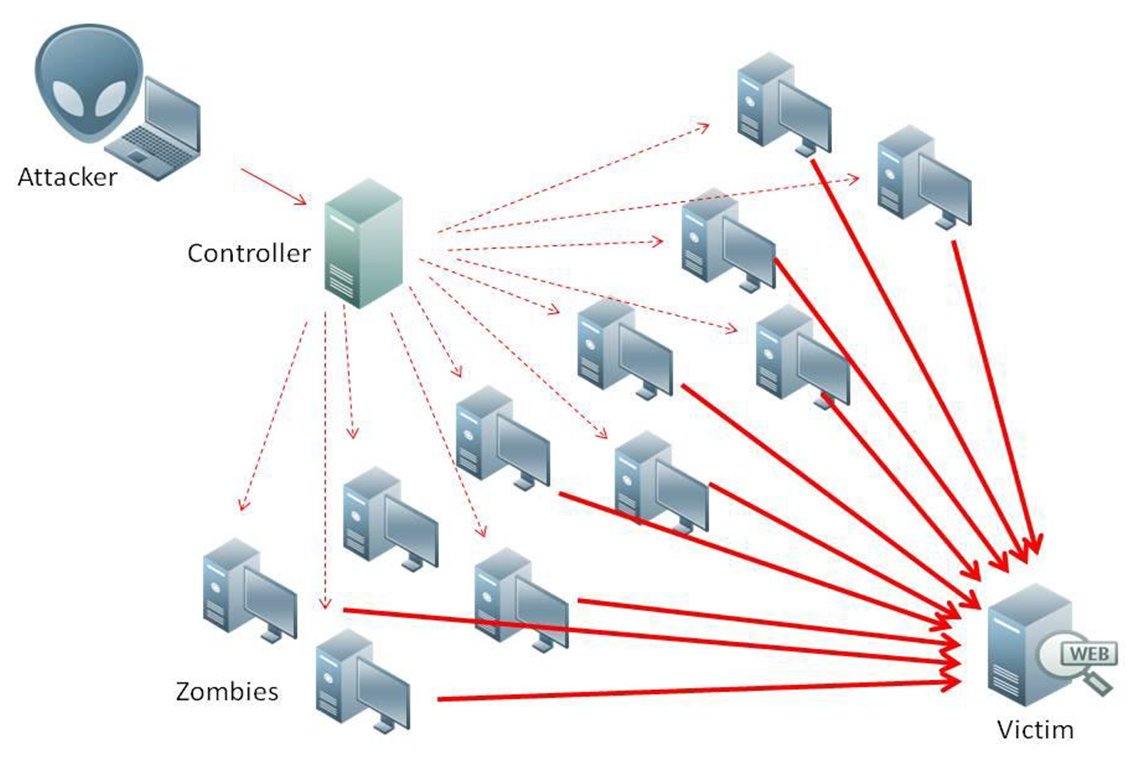
\includegraphics[width=0.7\linewidth]{ddos-attack-ex}
	\label{fig:ddos-attack-ex}
\end{figure}
\center \tiny Fonte: Wikipedia

\end{frame}

\begin{frame}{Exemplos de ataques: MITM}
	Man in the Middle
	\begin{itemize}	
		\item Alguém pelo meio
	\end{itemize}
	
	\begin{figure}
		\centering
		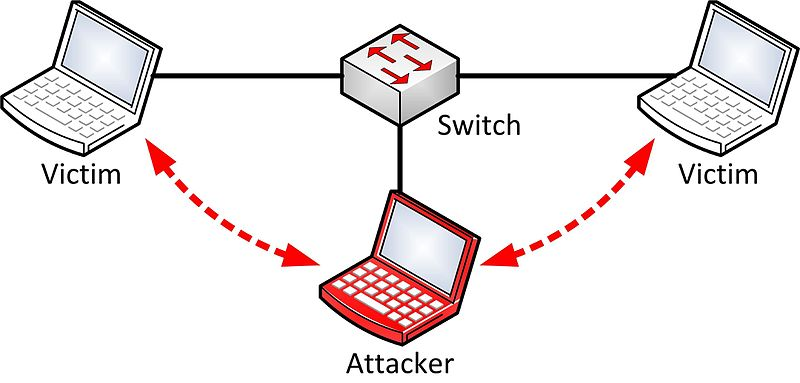
\includegraphics[width=0.7\linewidth]{mitm}
		\label{fig:mitm-attack-ex}
	\end{figure}
	\center \tiny Fonte: Wikipedia
	
\end{frame}

\section{Ataques famosos}

\begin{frame}{Ataques Famosos}
	\begin{itemize}
		\item \href{http://www.businessinsider.com/hackers-use-a-refridgerator-to-attack-businesses-2014-1}{Pela primeira vez, hackers utilizaram refrigeradores para atacar empresas}
		\item \href{http://www.theage.com.au/it-pro/security-it/cyber-attack-that-sent-750k-malicious-emails-traced-to-hacked-refrigerator-tvs-and-home-routers-20140120-hv96q.html}{Ataques cibernéticos enviam mais de 750k emails maliciosos a partir de refrigeradores, TVs e roteadores hackeados}
		\item \href{http://www.theregister.co.uk/2015/08/24/smart_fridge_security_fubar/}{Geladeira inteligente da Samsung deixa credenciais de login no Gmail livre para ataque}
		\item \href{http://www.theguardian.com/technology/2015/jul/21/jeep-owners-urged-update-car-software-hackers-remote-control}{Donos de carros da marca Jeep são contactados para atualizar software de seus veículos após hackers conseguirem controle remoto completo}
		\item \href{https://www.theguardian.com/technology/2015/nov/26/hackers-can-hijack-wi-fi-hello-barbie-to-spy-on-your-children}{Hackers conseguem injetar códigos em Boneca da Barbie e espionam crianças}
	\end{itemize}	
\end{frame}

\section{Vulnerabilidades}

\begin{frame}{Vulnerabilidades}
Categorias de vulnerabilidades (parte 1)
% Fonte: https://www.owasp.org/images/8/8e/Infographic-v1.jpg
\begin{itemize}
	\item Interface Web insegura
	\item Autenticação e Autorização insuficiente
	\item Serviços de rede inseguros
	\item Falta de encriptação no transporte de dados
	\item Preocupação com privacidade
\end{itemize}
\end{frame}

\begin{frame}{Vulnerabilidades}
Categorias de vulnerabilidades (parte 2)
% Fonte: https://www.owasp.org/images/8/8e/Infographic-v1.jpg
\begin{itemize}
	\item Interface de Cloud insegura
	\item Interface Mobile insegura
	\item Configurabilidade da segurança insegura
	\item Insegurança de software/firmware
	\item Segurança física pobre
\end{itemize}
\end{frame}


\begin{frame}{Segurança de dados}
Tipos de Segurança Básica (parte 1)
% Fonte: http://blog.gemalto.com/wp-content/uploads/2014/04/Gemalto-Top10Security-Infographic_FINAL-resized1.jpg
\begin{itemize}
	\item Métodos fortes de autenticação
	\item Atualização de softwares
	\item Segurança física de equipamentos e portas
	\item Estabelecer política de segurança para usuários
	\item Encriptar dados
\end{itemize}
\end{frame}

\begin{frame}{Segurança de dados}
Tipos de Segurança Básica (parte 2)
\begin{itemize}
\item Proteger dispositivos contra vírus
\item Proteger a rede de acesso externo
\item Executar auditoria interna de segurança
\item Definir regras mais rígidas para administradores
\item Avaliar política de uso de dispositivos pessoais e protocolo BYOD (\textit{bring your own device}) da organização
\end{itemize}
\end{frame}

\frame{\titlepage}

\end{document}
